%% ****** Start of file apstemplate.tex ****** %
%%
%%
%%   This file is part of the APS files in the REVTeX 4 distribution.
%%   Version 4.1 of REVTeX, October 2009
%%
%%
%%   Copyright (c) 2001, 2009 The American Physical Society.
%%
%%   See the REVTeX 4 README file for restrictions and more information.
%%
%
% This is a template for producing manuscripts for use with REVTEX 4.0
% Copy this file to another name and then work on that file.
% That way, you always have this original template file to use.
%
% Group addresses by affiliation; use superscriptaddress for long
% author lists, or if there are many overlapping affiliations.
% For Phys. Rev. appearance, change preprint to twocolumn.
% Choose pra, prb, prc, prd, pre, prl, prstab, prstper, or rmp for journal
%  Add 'draft' option to mark overfull boxes with black boxes
%  Add 'showpacs' option to make PACS codes appear
%  Add 'showkeys' option to make keywords appear
\documentclass[aps,pra,amsmath,amssymb,preprint,groupedaddress]{revtex4}
%\documentclass[aps,prl,preprint,superscriptaddress]{revtex4-1}
%\documentclass[aps,prl,reprint,groupedaddress]{revtex4-1}

% You should use BibTeX and apsrev.bst for references
% Choosing a journal automatically selects the correct APS
% BibTeX style file (bst file), so only uncomment the line
% below if necessary.
%\bibliographystyle{apsrev4-1}
\usepackage{graphicx}
\usepackage{epstopdf}
\usepackage{subfig}

%\usepackage{setspace}\doublespace

\newcommand{\vk}{\ensuremath{\mathbf{k}}}
\providecommand{\vr}{\ensuremath{\mathbf{r}}}
%\newcommand{\vec}[1]{\ensuremath{\mathbf{#1}}}

\newcommand{\gk}{\ensuremath{{g}(\mathbf{k})}}

\newcommand{\vp}{\ensuremath{\mathbf{p}}}
\newcommand{\gp}{\ensuremath{{g}(\mathbf{p})}}

\newcommand{\vq}{\ensuremath{\mathbf{q}}}

\newcommand{\Fo}{\ensuremath{\mathbf{F_0}}}


\newcommand{\E}{\ensuremath{\mathbf{E}}}
\newcommand{\A}{\ensuremath{\mathbf{A}}}
\newcommand{\J}{\ensuremath{\mathcal{J}}}

\newcommand{\ket}[1]{\ensuremath{\left|#1\right>}}
\newcommand{\bra}[1]{\ensuremath{\left<#1\right|}}

\newcommand{\twoe}{\ensuremath{2\epsilon_\vk-\E_1}}

\newcommand{\nth}[1]{\ensuremath{\frac{1}{#1}}}

\newcommand{\br}[1]{\ensuremath{\left(#1\right)}}
\newcommand{\mbr}[1]{\ensuremath{\left[#1\right]}}
\newcommand{\bbr}[1]{\ensuremath{\left\{#1\right\}}}


\newcommand{\tk}{\ensuremath{\tilde{k}}}

\newcommand{\kp}{\ensuremath{\ket{\Psi}}}

\newcommand{\av}[1]{\ensuremath{\bigl<{#1}\bigr>}}
\newcommand{\avv}[2][\nu]{\av{#1{\lvert{#2}\rvert}#1}}
\newcommand{\avt}[2]{\av{{#1}|{#2}}}
\newcommand{\avtu}[1]{\av{T_\tau#1}}

\newcommand{\Bop}{\ensuremath{\mathbf{B_0^+}}}
\newcommand{\Bmp}{\ensuremath{\mathbf{B_m^+}}}
\newcommand{\Bnp}{\ensuremath{\mathbf{B_n^+}}}
\newcommand{\Bo}{\ensuremath{\mathbf{B_0}}}
\newcommand{\Bopn}{\ensuremath{\mathbf{{B_0^+}^n}}}
\newcommand{\Bon}{\ensuremath{\mathbf{{B_0}^n}}}


\newcommand{\zmatrix}{\ensuremath{\br{\begin{smallmatrix}0&0\\0&0\end{smallmatrix}}}}
\newcommand{\fmtrx}[4]{\ensuremath{\br{\begin{smallmatrix}#1&#2\\#3&#4\end{smallmatrix}}}}
\newcommand{\smtrx}[6]{\ensuremath{\br{\begin{smallmatrix}#1&#2\\#3&#4\\#5&#6\end{smallmatrix}}}}

\newcommand{\vz}{\ensuremath{v^{\beta\alpha}_{\vk,\vk}}}
%\newcommand{\fz}{

\providecommand{\abs}[1]{\ensuremath{\lvert{#1}\rvert}}

\newcommand{\sg}[1][1]{\ensuremath{\sigma_\frac{#1}{2}}}

\newcommand{\rhof}{\ensuremath{\rho(\ef)}}
\newcommand{\omt}{\ensuremath{\tilde{\Omega}}}
\newcommand{\cht}{\ensuremath{\tilde{\chi_0}}}
\newcommand{\Atl}{\ensuremath{\abs{A}^{2l}}}
\newcommand{\ef}{\ensuremath{\epsilon_F}}

\newcommand{\lca}{\ensuremath{\ln\br{1+\frac{\cht}{\alpha}}}}

\newcommand{\com}[2]{\ensuremath{\mbr{#1,#2}}}
\newcommand{\D}{\ensuremath{\mathit{D}}}
\newcommand{\dg}{\ensuremath{\dagger}}

\providecommand{\lvk}{\ensuremath{1/\vk_F}}
\providecommand{\hm}{\ensuremath{\frac{\hbar^2}}{2m}}
\providecommand{\pdiff}[2]{\ensuremath{\frac{\partial{#1}}{\partial{#2}}}}
\providecommand{\dpdiff}[2]{\ensuremath{\frac{\partial^2{#1}}{\partial{{#2}^2}}}}

\providecommand{\H}{\ensuremath{\mathcal{H}}}
\providecommand{\wt}[1]{\widetilde{#1}}


\begin{document}

% Use the \preprint command to place your local institutional report
% number in the upper righthand corner of the title page in preprint mode.
% Multiple \preprint commands are allowed.
% Use the 'preprintnumbers' class option to override journal defaults
% to display numbers if necessary
%\preprint{}

\title{Coboson Approach to
 Cooper Pairs}
%Title of paper

% repeat the \author .. \affiliation  etc. as needed
% \email, \thanks, \homepage, \altaffiliation all apply to the current
% author. Explanatory text should go in the []'s, actual e-mail
% address or url should go in the {}'s for \email and \homepage.
% Please use the appropriate macro foreach each type of information

% \affiliation command applies to all authors since the last
% \affiliation command. The \affiliation command should follow the
% other information
% \affiliation can be followed by \email, \homepage, \thanks as well.
\author{Guojun Zhu}

%\email[]{Your e-mail address}
%\homepage[]{Your web page}
%\thanks{}
%\altaffiliation{}
\affiliation{}
\author{Monique Combescot}
%Collaboration name if desired (requires use of superscriptaddress
%option in \documentclass). \noaffiliation is required (may also be
%used with the \author command).
%\collaboration can be followed by \email, \homepage, \thanks as well.
%\collaboration{}
%\noaffiliation

\date{\today}

\begin{abstract}
% insert abstract here
\end{abstract}

% insert suggested PACS numbers in braces on next line
\pacs{}
% insert suggested keywords - APS authors don't need to do this
%\keywords{}

%\maketitle must follow title, authors, abstract, \pacs, and \keywords
\maketitle

% body of paper here - Use proper section commands
% References should be done using the \cite, \ref, and \label commands
\section{Basic Coboson Formalism}
We consider pairs of opposite spin electrons with zero total momentum.  These electrons interact through the standard BCS potential that we take here as granted without discussing its oversimplification. This potential reads as 

\begin{equation}\label{eq:vbcs}
V_{BCS}=\sum{v_{\vk'\vk}\beta^+_{\vk'}\beta^{}_{\vk}}
\end{equation}
where $v_{\vk'\vk}$ is taken as a separable potential, $v_{\vk'\vk}=-V\,w_{\vk'}w_{\vk}$ with $V$ being a small positive constant.  $\beta^+_\vk=a^+_{\vk\uparrow}a^+_{-\vk\downarrow}$ creates a pair of opposite spin electrons with momentum $\br{\vk,-\vk}$ while $w_\vk$ is equal to 1 for electrons in the energy layer where the potential acts. This layer lies above a Fermi sea $\ket{F_0}$ full of electrons which are thus "frozen" with respect to the $V_{BCS}$ potential.  Electrons feeling this potential have an energy $\epsilon_\vk$ such that,  $\epsilon_{F_0}<\epsilon_\vk<\epsilon_{F_0}+\Omega$. Scattering processes induced by the BCS potential given in eq \eqref{eq:vbcs} are represented in fig (\ref{fig:direct}).  The BCS hamiltonian for up and down spin electrons then reads as $H_{BCS}=H_0+V_{BCS}$, the free part $H_0$ being given by
\begin{equation}
H_0=\sum{\epsilon_\vk\br{a^+_{\vk\uparrow} a^{}_{\vk\uparrow}+a^+_{-\vk\downarrow} a^{}_{-\vk\downarrow}}}
\end{equation}

 The coboson formalism \cite{CobosonPhysicsReports} originally developed for composite bosons  made of two fermions like  excitons or Hydrogen atoms, relies on an operator algebra made of commutators.  This algebra has to be contrasted with the scalar algebra made of Green functions developed for elementary quantum particles.  The main advantage of this operator algebra is to possibly deal with the Pauli exclusion principle between the particle fermionic components in an exact way.  A few elementary commutators between free electron pairs are necessary to construct the formalism adapted to Cooper pair composite bosons.  Let us calculate them first.

\subsection{Commutators for free electron pairs}

From the anticommutators of electron operators $\bbr{a^+_{\vk'{}s'},a^+_{\vk{}s}}=a^+_{\vk'\,s'}a^+_{\vk,s}+a^+_{\vk{}s}a^+_{\vk'{}s'}=0$ and $\bbr{a^{}_{\vk'{}s'},a^+_{\vk{}s}}=\delta_{\vk'\vk}\delta_{s'\,s}$, it is easy to show that the commutators for fermion pair creation operators as $\com{\beta^+_{\vk'}}{\beta^+_{\vk}}=\beta^+_{\vk'}\beta^+_{\vk}-\beta^+_{\vk}\beta^+_{\vk'}$ reduces to zero. Let us however note that $\br{a^+_{\vk,s}}^2=0$ simply follows from  $\bbr{a^+_{\vk,s},a^+_{\vk,s}}=0$, the cancellation of $\br{\beta^+_{\vk}}$ does not follow from $\com{\beta^+_{\vk}}{\beta^+_{\vk}}=0$, but from the fact that  $\br{\beta^+_{\vk}}^2$ contains $\br{a^+_{\vk{}s}}^2$.  The cancellation of $\br{\beta^+_{\vk}}^2$ seems to be lost when turning from electron operators $\br{a^+_{\vk\uparrow},a^+_{-\vk\downarrow}}$ to pair operators  $\beta^+_\vk$. We will see below that the relation $\br{\beta^+_{\vk}}^2=0$, which comes from Pauli blocking, is in fact preserved in the commutation algebra of these electron pairs. 

If we now consider creation and annihilation operators, we find
\begin{equation}\label{eq:betacom}
\com{\beta_{\vk'}}{\beta^+_{\vk}}=\delta_{\vk'\vk}-\D_{\vk'\vk}
\end{equation}
\begin{equation}\label{eq:D}
\D_{\vk'\vk}=\delta_{\vk'\vk}\br{a^+_{\vk\uparrow}a^{}_{\vk\uparrow}+a^+_{-\vk\downarrow}a^{}_{-\vk\downarrow}}
\end{equation}
The operator $\D_{\vk'\vk}$ would reduce to  zero if electron pairs were elementary bosons. By noting that
\begin{subequations}
\begin{equation}
\com{a^+_{\vk\uparrow}a^{}_{\vk\uparrow}}{\beta^+_{\vp}}=\delta_{\vk\vp}\beta^+_{\vp}=\com{a^+_{-\vk\downarrow}a^{}_{-\vk\downarrow}}{\beta^+_{\vp}}
\end{equation}
it is easy to show that 
\begin{equation}\label{eq:Dcom}
\com{\D_{\vk'_1\vk_1}}{\beta^+_{\vk_2}}=2\beta^+_{\vk_2}\delta_{\vk_1\vk_2}\delta_{\vk'_1,\vk_2}
\end{equation}
\end{subequations}
This leads us to identify  the exchange scattering for free electron pairs, formally defined by 
\begin{equation}
\com{\D_{\vk'_1\vk_1}}{\beta^+_{\vk_2}}=\sum_{\vk'_2}\bbr{\lambda\fmtrx{\vk'_2}{\vk_2}{\vk'_1}{\vk_1}+\br{\vk'_1\leftrightarrow\vk'_2}}\beta^+_{\vk'_2}
\end{equation}
with a product of Kronecker symbols 
\begin{equation}\label{eq:pauliscattering}
\lambda\fmtrx{\vk'_2}{\vk_2}{\vk'_1}{\vk_1}=\delta_{\vk'_1\vk_1}\delta_{\vk'_2\vk_2}\delta_{\vk_1\vk_2}
\end{equation}
Actually, this is just the value we expect for the scattering associated to electron exchanges between $\br{\vk_1,\vk_2}$ pairs, as visualized by the diagram of fig (\ref{fig:lambda}).

The link between this exchange scattering and the Pauli exclusion principle can be easier to see if we  consider the scalar product of two electron pairs.  Indeed, using these commutators, we find
\begin{equation}\label{eq:4beta}
\begin{split}
\av{v\abs{\beta_{\vk'_1}\beta_{\vk'_2}\beta^+_{\vk_2}\beta^+_{\vk_1}}v}&=\bbr{\delta_{\vk'_1\vk_1}\delta_{\vk'_2\vk_2}-\lambda\fmtrx{\vk'_2}{\vk_2}{\vk'_1}{\vk_1}}+\br{\vk'_1\leftrightarrow\vk'_2}\\
&=\delta_{\vk'_1\vk_1}\delta_{\vk'_2\vk_2}\br{1-\delta_{\vk_1\vk_2}}+\br{\vk'_1\leftrightarrow\vk'_2}
\end{split}
\end{equation}
The above result readily shows that the Pauli scattering $\lambda\fmtrx{\vk'_2}{\vk_2}{\vk'_1}{\vk_1}$ insure the RHS to cancel for $\vk_1=\vk_2$, as necessary from Pauli blocking in the LHS, the state $\beta^+_{\vk_2}\beta^+_{\vk_1}\ket{v}$ reducing to zero when $\vk_1=\vk_2$.

We now consider the commutator of the free pair creation operator $\beta^+_\vp$ with the BCS hamiltonian.  Using eq. \eqref{eq:Dcom}, we find for the free part
\begin{equation}\label{eq:betaH}
\com{H_0}{\beta^+_\vp}=2\epsilon_\vp\beta^+_\vp
\end{equation}
while the potential part gives 
\begin{equation}\label{eq:vbeta}
\com{V_{BCS}}{\beta^+_\vp}=\gamma^+_\vp+V^+_\vp
\end{equation}
where we have set $\gamma^+_\vp=\sum_\vk\beta^+_\vk{}v_{\vk\vp}$. The "creation potential" for the free pair $\vp$ appears to be 
\begin{equation}\label{eq:betaV}
V^+_\vp=-{\gamma^+_\vp}\br{a^+_{\vp\uparrow}a^{}_{\vp\uparrow}+a^+_{-\vp\downarrow}a^{}_{-\vp\downarrow}}
\end{equation}
While the $\gamma^+_\vp$ part of \com{V_{BCS}}{\beta^+_\vp} commutes with $\beta^+_\vp$, the creation potential $V^+_\vp$ does not.  Its commutator precisely reads
\begin{equation}\label{eq:vpotbeta}
\com{V^+_{\vp_1}}{\beta^+_{\vp_2}}=-2\delta_{\vp_1\vp_2}\gamma^+_{\vp_1}\beta^+_{\vp_1}
\end{equation}

This allows us to identify the interaction scattering for free pairs, formally defined as 
\begin{equation}
\com{V^+_{\vp_1}}{\beta^+_{\vp_2}}=\sum\chi\fmtrx{\vp'_2}{\vp_2}{\vp'_1}{\vp_1}\beta^+_{\vp'_1}\beta^+_{\vp'_2}
\end{equation}
with a sequence of exchanged and scattering
\begin{equation}\label{eq:interactSc}
\begin{split}
\chi\fmtrx{\vp'_2}{\vp_2}{\vp'_1}{\vp_1}&=-\sum_\vk\bbr{v_{\vp'_1\vk}\lambda\fmtrx{\vp'_2}{\vp_2}{\vk}{\vp_1}+\br{\vp'_1\leftrightarrow\vp'_2}}\\
&=-\br{v_{\vp'_1,\vp_1}\delta_{\vp'_2,\vp_2}+v_{\vp'_2,\vp_2}\delta_{\vp'_1,\vp_1}}\delta_{\vp_2,\vp_1}
\end{split}
\end{equation}
This interaction scattering is visualized by  the diagram of fig \ref{fig:chi}: the two free pairs $\vp'_1$ and $\vp'_2$ first exchange an electron; as for any exchange, this brings a minus sign.  In a second step, one of the two pairs interact via the BCS potential.  

Using these commutators, it is easy to find $V_{BCS}$ acting on free pair states.  By noting that $V^+_\vp\ket{F_0}=0$ due to the factor $v_{\vk\vp}=-V\,w_\vk{}w_\vp$  included is $\gamma^+_\vp$, we find for one-free-pair state:
\begin{equation}
V_{BCS}\beta^+_\vp\ket{F_0}=\gamma^+_\vp\ket{F_0}
\end{equation}
For two-free-pair state,  eqs. (\ref{eq:vbeta},\ref{eq:vpotbeta}) give

\begin{equation}\label{eq:vbcs2}
\begin{split}
V_{BCS}\beta^+_{\vp_1}\beta^+_{\vp_2}\ket{F_0}&=\br{\gamma^+_{\vp_1}\beta^+_{\vp_2}+\beta^+_{\vp_1}\gamma^+_{\vp_2}+\sum\chi\fmtrx{\vp'_2}{\vp_2}{\vp'_1}{\vp_1}\beta^+_{\vp'_2}\beta^+_{\vp'_2}}\ket{F_0}\\
&=\br{\gamma^+_{\vp_1}\beta^+_{\vp_2}+\beta^+_{\vp_1}\gamma^+_{\vp_2}-2\delta_{\vp_1\vp_2}\gamma^+_{\vp_1}\beta^+_{\vp_1}}\ket{F_0}
\end{split}
\end{equation}
and so on... The above equation tells us that the two pairs of a two-free-pair state do not interact except through the Pauli exclusion principle.  This Pauli blocking appears through the $\delta_{\vp_1\vp_2}$ term in eq. \eqref{eq:vbcs2}. It just insures the RHS to cancel when  $\vp_1=\vp_2$ as necessary since ${\beta^+_\vp}^2=0$ due to the Pauli exclusion principle between up or down spin electrons.% ??? of $V_{BCS}$, electrons can interact through Pauli blocking only, will appear in an even more ??? way in terms of Cooper pair operator as done in the next section.  

 \begin{figure}[htb]
 \centering
 \subfloat[][]{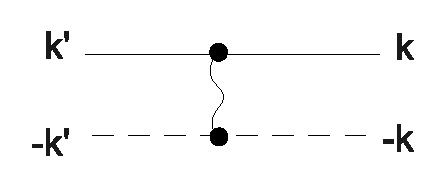
\includegraphics{cobosonCooper/direct1}\label{fig:direct}}\qquad
 \subfloat[][]{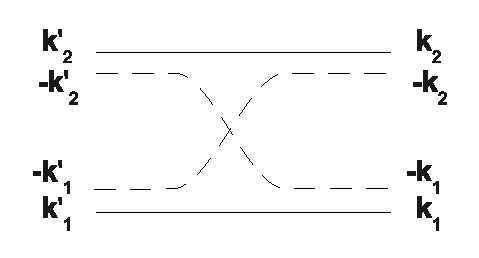
\includegraphics{cobosonCooper/lambda1}\label{fig:lambda}}\\
 \subfloat[][]{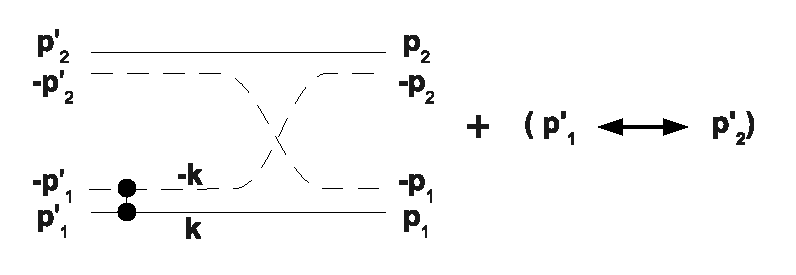
\includegraphics[width=0.8\textwidth]{cobosonCooper/chi1}\label{fig:chi}}  + \qquad $\br{\vp'_1\leftrightarrow\vp'_2}$
 \caption{Shiva diagram of free pairs }


 \begin{description}
 \item[\subref{fig:direct}] The BCS potential given in eq. \eqref{eq:vbcs} transforms a $\vk$ pair into a $\vk'$ pair, with a constant scattering $-V$, in the case of separable potential $v_{\vk'\vk}=-V\,w_{\vk'}w_{\vk}$. Up spin electrons are represented by solid line while down spin electrons are represented by dashed line.
 
 \item[\subref{fig:lambda}] Pauli scattering $\lambda\fmtrx{\vp'_2}{\vp_2}{\vp'_1}{\vp_1}$ for electron exchange between two free pairs $\br{\vp_1,\vp_2}$, as given by eq. \eqref{eq:pauliscattering}.
 
 \item[\subref{fig:chi}] Interaction scattering  $\chi\fmtrx{\vp'_2}{\vp_2}{\vp'_1}{\vp_1}$ between two free electron pairs, as given in eq \eqref{eq:interactSc}. Since the BCS potential acts within one pair only, the interaction between two pairs come from exchange induced by the Pauli exclusion principle.
 \end{description} 


 \end{figure}



\subsection{Cooper pair creation operators}

We now introduce the linear combinations of free pairs creation operators which are the one-pair eigenstates of the BCS hamiltonian.  These operators create the Cooper pair states $\ket{i}=B^+_i\ket{F_0}$ where $\ket{F_0}$ is the "frozen" Fermi sea. Note that these Cooper pairs states not only include the standard ground state for single pair derived by Cooper, but also all the one-pair excited states in order to form a complete set for electron pairs with zero total momentum.  The closure relations written with free pairs and Cooper pairs then read, for normalized  states $\ket{i}$, i.e., states such that $\avt{i}{i}=1$
\begin{equation}\label{eq:enclosureK}
I=\sum_\vk{\beta^+_\vk\ket{F_0}\bra{F_0}\beta^{}_\vk}
\end{equation}
\begin{equation}
I=\sum_i{B^+_i\ket{F_0}\bra{F_0}B^{}_i}
\end{equation}
By injecting eq. \eqref{eq:enclosureK} in front of $\ket{i}$, it is then easy to show that free pair and Cooper pair creator operators, $\beta^+_\vk$ and $B^{}_i$ are linked by 
\begin{equation}\label{eq:bbeta}
B^{+}_i=\sum_\vk{\beta^+_\vk\avt{\vk}{i}}
\end{equation}
\begin{equation}
\beta^+_\vk=\sum_iB^{+}_i{\avt{i}{\vk}}
\end{equation}
where $\ket{\vk}=\beta^+_\vk\ket{F_0}$ is the single free pair state made of the frozen Fermi sea $\ket{F_0}$ plus one free electron pair $\br{\vk,-\vk}$. Note that $\ket{\vk}$ differs from zero for $\epsilon_\vk$ larger than the frozen Fermi sea energy $\epsilon_{F_0}$.
\subsection{Commutation for Cooper pair operators}

Using the commutators for free electron pairs given in eqs. (\ref{eq:betacom},\ref{eq:D}), it is easy to show that for normalized Cooper pair eigenstates $\avt{i}{j}=\delta_{ij}$, we do have 
\begin{equation}\label{eq:bcom}
\com{B_m}{B^+_i}=\delta_{mi}-\D_{mi}
\end{equation}
\begin{equation}
\begin{split}
\D_{mi}&=\sum_\vk{\avt{m}{\vk}\D_{\vk\vp}\avt{\vp}{i}}\\
			&=\sum_\vk{\avt{m}{\vk}\avt{\vk}{i}}\br{a^+_{\vk\uparrow}a^{}_{\vk\uparrow}+a^+_{-\vk\downarrow}a^{}_{-\vk\downarrow}}
\end{split}
\end{equation}
Note that due to the $\ket{\vk}$ state in the prefactor,  the relavant  $\vk$ electrons in the sum are above $\ket{F_0}$, so that $\D_{mi}\ket{F_0}=0$.  Pauli scattering for Cooper pairs follows as

\begin{equation}
\com{\D_{mi}}{B^+_j}=2\sum_{n}\lambda\fmtrx{n}{j}{m}{i}B^+_{n}
\end{equation}
\begin{equation}\label{eq:blambda}
\lambda\fmtrx{n}{j}{m}{i}=\sum_\vk\avt{m}{\vk}\avt{n}{\vk}\avt{\vk}{i}\avt{\vk}{j}
\end{equation}
This Pauli scattering is visualized by the diagram of fig (\ref{fig:blambda}). This diagram is the same structure as the Shiva diagram for carrier exchanges we introduced in the many-body theory of composite boson excitons. 

From these commutators, we readily find that the scalar product of two Cooper pair states has the usual form, namely
\begin{equation}\label{eq:4B}
\av{F_0\abs{B_mB_nB^+_jB^+_i}v}=\delta_{mi}\delta_{nj}+\delta_{mj}\delta_{ni}-2\lambda\fmtrx{n}{j}{m}{i}
\end{equation}
By noting that $\avt{m}{i}=\sum_\vk{\avt{m}{\vk}\avt{\vk}{i}}$, we can rewrite this scalar product, using the expression of the Pauli scattering given in eq. \eqref{eq:blambda}, as 
\begin{equation}\label{eq:4B2}
\av{F_0\abs{B_mB_nB^+_jB^+_i}v}=\sum_\vk{\avt{m}{\vk}\avt{\vk}{i}}\sum_{\vk'\neq\vk}{\avt{n}{\vk'}\avt{\vk'}{j}}+\br{m\leftrightarrow{n}}
\end{equation}
The above expression shows in a quite clear way that the effects of the $\lambda\fmtrx{n}{j}{m}{i}$ term in the scalar product \eqref{eq:4B} is just to remove $\vk'=\vk$ terms from the sum, as a result of the Pauli exclusion principle between electrons making the Cooper pairs. However, from a technical point of view, the expression of Cooper pair scalar products with restricted sums, like the one of eq \eqref{eq:4B2}, are less convenient to handle than expressions using $\lambda\fmtrx{n}{j}{m}{i}$ like the one of eq. \eqref{eq:4B}.  This is why the introduction of Pauli scatterings to take care of the Pauli exclusion principle is indeed convenient, mostly when the number of Cooper pair at hand is large.

Let us now turn to the interaction scatterings between Cooper pairs. For that, we first note that for $\ket{i}$ being hamiltonian eigenstates, we do have, by inserting $I=\sum\ket{\vp}\bra{\vp}$ in front of $\ket{i}$

\begin{equation}
0=\br{H-E_i}\ket{i}=\sum_\vp\avt{\vp}{i}\mbr{\br{2\epsilon_\vp-E_i}\beta^+_\vp+\sum_\vk\beta^+_\vk{}v_{\vk\vp}}\ket{F_0}
\end{equation}  
If we now  project the above equation on $\bra{\vp'}$, we find since $\avt{\vp'}{\vp}=\delta_{\vp'\vp}$ that the $\avt{\vp}{i}$'s fulfill the Schr\"{o}dinger equation
\begin{equation}\label{eq:sch}
2\epsilon_\vp\avt{\vp'}{i}+\sum_\vp{v_{\vp'\vp}\avt{\vp}{i}}=E_i\avt{\vp'}{i}
\end{equation}
This equation gives $\avt{\vp'}{i}$ in terms of a sum of $\avt{\vp}{i}$. From it, we do recover, in the case of a separable potential $v_{\vp'\vp}=-V\,w_\vp{}w_{\vp'}$,  the well-known equation  of the one-Cooper pair energy, namely
\begin{equation}
\nth{V}=\sum\frac{w_\vp}{2\epsilon_\vp-E_i}
\end{equation}
Using eq  \eqref{eq:sch}, it is then easy to show, from eqs (\ref{eq:4beta},\ref{eq:betaH}) that the commutator $\com{H_0}{B^+_i}$ has the standard form, namely
\begin{equation}
\begin{split}
\com{H}{B^+_i}&=\sum_\vp\avt{\vp}{i}\br{2\epsilon_\vp\beta^+_\vp+\sum_\vk\beta^+_\vk{}v_{\vk\vp}}+V^+_\vp\\
&=E_iB^+_i+V^+_i
\end{split}
\end{equation}
where $V^+_i=\sum\avt{\vp}{i}V^+_\vp$. Using the definition of $V^+_\vp$ given in eq \eqref{eq:vbeta}, we then find that 
\begin{equation}
\com{V^+_i}{B^+_j}=-2\sum_{\vp\vk}\avt{\vp}{i}\avt{\vp}{j}\beta^+_\vp\beta^+_\vk{}v_{\vk\vp}
\end{equation}
If we now use eq \eqref{eq:bbeta} to write free pair operators in term of Cooper pair and symmetrize the result with respect to $m$ and $n$, we end with
\begin{equation}
\com{V^+_i}{B^+_j}=\sum_{mn}\chi\fmtrx{n}{j}{m}{i}B^+_nB^+_m
\end{equation}
where the interaction scattering is given by
\begin{equation}\label{eq:bchi}
\chi\fmtrx{n}{j}{m}{i}=-\sum_{\vk\vp}{\avt{m}{\vk}\avt{n}{\vp}\avt{\vp}{j}\avt{\vp}{i}v_{\vk\vp}}+\br{m\leftrightarrow{n}}
\end{equation}
This scattering is represented by the diagram of fig (\ref{fig:bchi}).

 \begin{figure}[htb]
 \centering
 
 \subfloat[][]{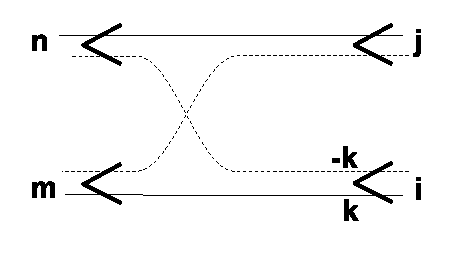
\includegraphics{cobosonCooper/BLambda}\label{fig:blambda}}\\
 \subfloat[][]{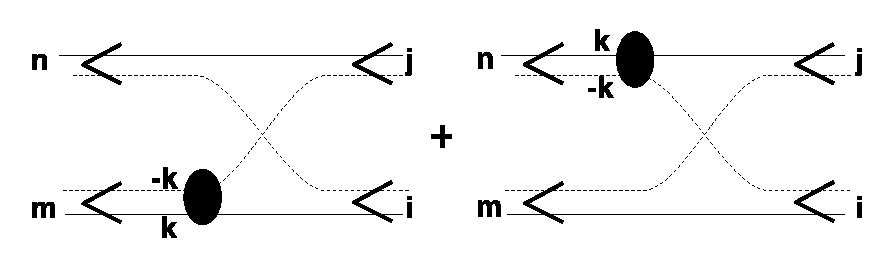
\includegraphics[width=0.8\textwidth]{cobosonCooper/BChi}\label{fig:bchi}}
 \caption{Shiva diagram of Cooper pairs }


 \begin{description}
 
 
 \item[\subref{fig:blambda}] Pauli scattering  for electron exchange between Cooper pair sas given by eq. \eqref{eq:blambda}.
 
 \item[\subref{fig:bchi}] Interaction scattering   between Cooper pairs, as given in eq. \eqref{eq:bchi}. Due to the peculiar form of the BCS potential, two Cooper pairs only interact through the Pauli exclusion principle, via electron exchange. 
 \end{description} 


 \end{figure}
\appendix
\section{On the possibility to rewrite the BCS hamiltonian in terms of Cooper pair operators}
Let us introduce the free pair hamiltonian defined as $\wt{H_0}=\sum{2\epsilon_\vk\beta^+_\vk\beta^{}_\vk}$.
This free pair hamiltonian and the free electron hamiltonian $H_0$ seems to act in the same way on n-pair states. Indeed, eq. \eqref{eq:4beta} gives $H_0$ acting on two pairs as 
\begin{equation}
\begin{split}
H_0\beta^+_{\vp_1}\beta^{}_{\vp_2}\ket{F_0}&=\br{\com{H_0}{\beta^+_{\vp_1}}+{\beta^+_{\vp_1}}{H_0}}\beta^{}_{\vp_2}\ket{F_0}\\
&=\br{2\epsilon_{\vp_1}+2\epsilon_{\vp_2}}\beta^+_{\vp_1}\beta^{+}_{\vp_2}\ket{F_0}
\end{split}
\end{equation}
In the case of $\wt{H_0}$, the same procedure gives with eq \eqref{eq:4beta} replaced by $\com{\wt{H_0}}{\beta^+_{\vp_1}}=2\epsilon_\vp\beta^+_\vp-\sum2\epsilon_\vk\beta^+_\vk{}\D_{\vk\vp}$
\begin{equation}
\br{\wt{H_0}-H_0}\beta^+_{\vp_1}\beta^{+}_{\vp_2}\ket{F_0}=-\sum2\epsilon_\vk\beta^+_\vk{}\D_{\vk\vp_1}\beta^{+}_{\vp_2}\ket{F_0}
\end{equation}
Due to eq \eqref{eq:D}, the RHS of the above equation reduces to zero for $\vp_1\neq\vp_2$.  Since this condition is fulfilled for the 2-pair state of interest in order for $\beta^+_{\vp_1}\beta^{+}_{\vp_2}\ket{F_0}$ to differ from zero  due to the Pauli exclusion principle, we are tempted to conclude that $H_0$ can be replaced by $\wt{H_0}$.

We can be even more tempted to make such a replacement once we note that $\wt{H}=\wt{H_0}+V_{BCS}$ takes a very compact form in term of Cooper pair operators. Indeed, we get using eq \eqref{eq:bbeta}.

\begin{equation}
\begin{split}
\wt{H}&=\sum_\vk\br{2\epsilon_\vk\beta^+_\vk+\sum_{\vk'}\beta^+_{\vp'}v_{\vp'\vp}}\beta^+_\vk\\	&=\sum_{ij}B^+_iB^{}_j\sum_\vk\mbr{2\epsilon_\vk\avt{i}{\vk}+\sum_{\vk'}\avt{i}{\vk'}v_{\vk'\vk}}\avt{\vk}{j}
\end{split}
\end{equation}
Since due to eq \eqref{eq:sch}, the bracket reduces to $E_i\avt{i}{\vk}$, the summation over $\vk$, performed through closure relation leads to 
\begin{equation}
\wt{H}=\sum{}E_iB^+_iB^{}_i
\end{equation}
In spite of the fact that $H_0$ and $\wt{H_0}$ act in a similar way on n-pair state, the replacement of $H_0$ by $\wt{H_0}$ introduce spurious Pauli blocking which ultimately affect all matrix elements.  To see it, we can note that

\begin{equation}
\begin{split}
\com{\wt{H_0}}{\beta^+_{\vp}}&=\sum2\epsilon_\vk\beta^+_\vk\com{\beta^{}_\vk}{\beta^+_\vp}\\
	&=2\epsilon_\vp\beta^+_\vp-\sum2\epsilon_\vk\beta^+_\vk{}\D_{\vk\vp}
\end{split}
\end{equation}
the first term in the RHS being the value of $\com{{H_0}}{\beta^+_{\vp}}$. Turning to Cooper pair operators, this leads to 
\begin{equation}
\com{\wt{H}}{B^+_i}=\com{{H}}{B^+_i}+W^+_i
\end{equation}
where $W^+_i=-\sum2\epsilon_\vk\beta^+_\vk{}\D_{\vk\vp}\avt{\vp}{i}$.  This additional operator $w^+_i$ in the commutator generates an additional contribution to the interaction scattering which then reads
\begin{equation}
\wt\chi\fmtrx{n}{j}{m}{i}=\chi\fmtrx{n}{j}{m}{i}-2\sum_{\vk\vp}2\epsilon_\vk{\avt{m}{\vk}\avt{n}{\vp}\avt{\vp}{j}\avt{\vp}{i}v_{\vk\vp}}
\end{equation}

If we now use the expression of $\chi\fmtrx{n}{j}{m}{i}$ given in eq \eqref{eq:bchi}, we find that the interaction scattering associated to $\wt{H}$ takes a quite compact form. Using eqs (\ref{eq:blambda},\ref{eq:sch}), we find
\begin{equation}
\begin{split}
\wt\chi\fmtrx{n}{j}{m}{i}&=-\sum_{\vk}\br{\sum_\vp\avt{m}{\vp}v_{\vp\vk}+2\epsilon_\vk\avt{m}{\vk}}\avt{n}{\vp}\avt{\vp}{j}\avt{\vp}{i}v_{\vk\vp}\\
&=-\br{E_m+E_n}\lambda\fmtrx{n}{j}{m}{i}
\end{split}
\end{equation}
Although somewhat nicer than the explicit expression of the interaction scattering $\chi\fmtrx{n}{j}{m}{i}$ given in eq \eqref{eq:sch}, it is however clear that the replacement of $H_0$ by  $\wt{H_0}$ brings spurious terms in the calculation.

All this once more show that the system hamiltonian written in terms of fermion operators cannnot be rewritten in terms of coboson operators, even when the potential is as simple as the BCS potential. 

\bibliography{citation}
\end{document}
